\chapter{竞价型云平台中在线服务的轻量级暖备机制}
\label{cha:gemini}

\section{本章概述}
\label{sec:gemini_intro}
随着信息技术的迅猛发展,人类的日常工作生活中已经习惯了无处不在、无所不能的互联网服务。很多互联网业务都要求 24 $\times$ 7(每时每刻在线)服务。同时,这些互联网服务还要求快速响应用户请求,例如:互联网视频直播,电子购物网站,社交网站等。这进一步要求后端服务(如:数据库服务或对象存储服务)的高可用性。通常观点认为要求高可用性的服务应该托管在专用服务器或可靠的虚拟机实例上,而不是使用竞价型实例。许多之前的研究工作 \cite{chohan2010see, Liu:2011:CMC:2170444.2170450, song2012optimal, Yi:2010:RCS:1844768.1845343, Andrzejak:2010:DMC:1906481.1906533} 持相同的观点和顾虑,聚焦于可中断的计算任务设计容错的策略或是修改已有的计算框架以适应竞价型实例的易失效特点。这些工作通过重新执行、任务检查点、负载迁移等技术手段来实现对竞价型实例失效的容错。然而,成本下降带来的巨大经济利益驱动着使用竞价型实例提供在线服务的研究工作。进来,He 等人的研究 \cite{He:2015:CCH:2749246.2749275} 已经表明使用竞价型实例提供互联网服务是可行的。他们的方法基于嵌套虚拟化和多种虚拟机迁移技术。

然而上述使用竞价型实例提供在线服务的研究工作有很大的局限性。基于虚拟机迁移技术的方法 \cite{He:2015:CCH:2749246.2749275} 面临着强制迁移导致的在线服务不可用。这类不可用问题出现在云平台回收竞价型实例的过程中。由于新的虚拟机实例启动和嵌套虚拟机迁移的时间通常超过云平台的告警时间,竞价型实例上托管的在线服务不得不承受这期间的不可用。即使虚拟机的快照操作通过时间可控的内存检查点技术 \cite{Singh:2013:YEG:2482626.2482642} 得以及时完成,在云平台中缺少底层虚拟机管理器支持的嵌套虚拟机进行延迟恢复也至少产生约 20 秒的服务停机时间 \cite{Hines:2009:PBL:1508293.1508301}。

除了强制性的不可用问题,性能也是在线服务提供商必须考虑的关键问题。更具体地说,在线服务性能的一个重要指标————响应时间对用户体验或者说 QoS 是尤为关键的。然而,已有的研究工作只关注在线服务的可用性和成本,而忽视了服务性能。基于嵌套虚拟化和虚拟机迁移技术的方法 \cite{He:2015:CCH:2749246.2749275} 对于计算密集的服务带来了不可接受的性能开销。嵌套虚拟化技术在支撑互联网服务时至多带来 50\% 的性能开销 \cite{He:2015:CCH:2749246.2749275},对于一些计算密集型的测试集,性能开销高达 68\% \cite{Williams:2012:XVO:2168836.2168849}。定期的内存检查点带来的运行时性能开销也有 15\% 左右 \cite{Sharma:2015:SDD:2741948.2741953}。此外出于避免数据和内存检查点数据丢失的考虑,He 等人的方法选择使用持久化的网络存储卷 EBS 而放弃了高性能的本地实例存储卷。然而对于很多在线服务来说,服务性能的瓶颈就在于底层存储的性能。

本章重新审视并探讨了使用竞价型实例提供高可用在线服务的问题。更进一步地,本章力求回答一个更有挑战性的问题:能否打破当前解决方法的局限性,使得使用竞价型实例部署的在线服务同时实现高可用性、高性能、低成本?本章提出了一个全新的基于暖备和互备技术的解决方法并实现了一个原型工具 \emph{Gemini}。\emph{Gemini} 拥有轻量级的服务迁移方法、时间可控的异步磁盘数据复制机制,和综合考虑市场价格及其稳定性的智能可用区选择策略。这里,术语``暖备'' 不同于 ``冷备'' 和 ``热备''。暖备是指用作备援的虚拟机实例一直处于运行状态,但主备节点的状态不是实时同步的。互备是指两个节点互相作为对方的备援节点,形成一个互备对。在线服务提供商可以在互备的两个节点上运行同一服务的两个分片或是不同服务组件。为使得这样一套机制正常运作,\emph{Gemini} 中包括三个不同的组成部分:一个部署于每个节点上的执行进程活迁移(Live Migration)和磁盘数据复制任务的代理,一个控制服务迁移和维护暖备、互备状态的迁移控制器,以及一个负责申请或购买新的虚拟机实例的节点调度器。通过使用暖备技术和轻量级服务迁移方法,申请新虚拟机实例和进行虚拟机快照的时间开销得以从服务迁移的关键路径中移除。因此,\emph{Gemini} 能够使用竞价型实例提供可用性更高的在线服务。通过改用轻量级的进程迁移技术,\emph{Gemini} 避免了嵌套虚拟化和虚拟机迁移带来的大量性能开销。通过时间可控的异步磁盘镜像机制,\emph{Gemini} 可以在保证服务可用性的同时使用虚拟机实例高性能的本地实例存储,获得数倍到数十倍于网络存储卷 EBS 的I/O性能。总的来说,本章的贡献主要包括:
\begin{enumerate}
\item 通过详细分析当前使用竞价型实例提供高可用服务的解决方法,指出了其主要缺陷是面临竞价型实例被回收时的强制性的服务不可用和多方面的性能限制。
\item 提出了新的使用竞价型实例提供在线服务的方法和框架 \emph{Gemini}。\emph{Gemini} 基于轻量级服务迁移方法和暖备、互备技术,能够根据价格趋势和稳定性灵活地选择可用区申请竞价型实例。
\item 实现了一个 \emph{Gemini} 的原型系统以验证其有效性。评测结果显示在相近的成本下相比之前的基于嵌套虚拟化和虚拟机的技术获得了显著的服务可用性和性能提升。
\end{enumerate}

\section{在线服务在竞价型云平台中的机遇和挑战}
\subsection{竞价型实例新特性和可用性限制}
2015 年 1 月,Amazon EC2 发布了一个竞价型实例的新特性 \cite{AWS_SITN:2016}:在竞价型实例被回收前两分钟,云租户可以收到一个告警通知。利用这个提前的告警通知,云租户可以针对竞价型实例被回收做一些紧急处理。这对在线服务来说是一个非常重要的变化。利用这个回收告警通知,在线服务有机会实现完全让用户感知不到的故障转移。这对于致力于提高可用性的在线服务提供商来说是非常有吸引力的。

在Amazon EC2,多个不同的地理区域有数十个完全隔离的可用区。不同可用区的竞价型实例属于不同的竞价型实例市场,一般会有着不同的市场价格。图 \ref{figure:sp} 所示是某一个可用区的 ``m3.medium'' 类型竞价型实例的价格历史,竞价型实例的价格通常保持在很低的位置,在云平台中计算资源不足的时候可能突然升高。在大部分时间,使用这样一个竞价型实例只需每小时少于一美分的价格。相对而言,一个相同硬件配置的按需型实例需要花费 6.7 美分每小时。当然,竞价型实例不总是比按需型实例便宜。目前的竞价价格设定上限是同配置类型按需型实例价格的10倍 \cite{AWS_SL:2014}。然而,竞价型实例的市场价格可能攀升到超出这个上限。在图中,可以看到每小时 0.7 美元的费率。也就是说,对于竞价型实例来说不可能通过设置一个非常高的竞价得到同按需型实例相同的可用性,云平台可能根据自身需要在某些时候回收掉某个可用区的全部竞价型实例。
\begin{figure}[]
  \centering
  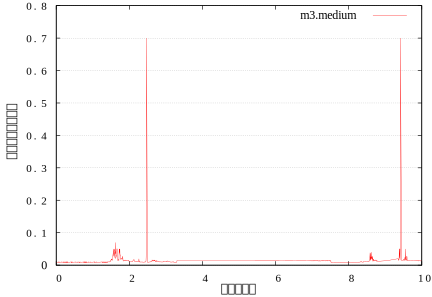
\includegraphics[width=0.9\textwidth]{spotprices}
  \caption{``us-west-2b'' 可用区的一个 ``linux.m3.medium'' 类型竞价型实例市场价格数据}
  \label{figure:sp}
\end{figure}

综上,对于在线服务提供商来说:竞价型云平台既提供了大幅降低计算成本的机会,也对在线服务的可用性造成了很大威胁。如何利用竞价型实例的新特性,实现竞价型实例上在线服务的高可用成为了在线服务提供商面临的主要挑战。

\subsection{云平台中的块存储设备}
Amazon EC2 云平台中有两种块存储设备:持久的网络存储卷和非持久的本地存储卷。使用持久的网络存储卷需要支付额外的费用,非持久的本地存储卷同虚拟机实例相关联不再需要支付额外的费用。临时的本地存储只在虚拟机实例的生命周期内有效,因为本地存储所在磁盘是直接连接在虚拟机所在的物理机上的。每种块设备存储都提供固态硬盘(SSD)和机械磁盘(HDD)两种选择。如表 \ref{table:ec2storage} 所示,非持久的本地实例存储在吞吐量和IOPS指标上都有更好的性能。SSD本地实例存储卷可以实现高达 100000 IOPS 的性能,是 EBS 存储卷的几个数量级。实例存储室完全免费的,因为在虚拟机实例的付费中已经包含这一部分。EBS 存储卷的费用是和它的性能成比例的。在 Amazon EC2 的 us-east1 区域的,通用型 EBS SSD 存储卷的价格每月每 GB 0.1 美元,预留 IOPS 的 EBS SSD 的成本是每月每 GB 0.125 美元以及每月每预留 IOPS 0.065 美元。使用高性能的 EBS SSD 将带来显著的额外成本。
\begin{table}
\centering
\begin{threeparttable}
\caption{Amazon EC2 存储性能比较}
\label{table:ec2storage}
\begin{tabular}{c|c|c} \hline
Storage Type& Throughput (MB/s)& IOPS (4KB)\\
\hline
Ephemeral SSD & 733 & 100,000\\
Persistent SSD 1 & 160 & 10,000\\
Persistent SSD 2 & 320 & 20,000\\
Ephemeral HDD & 110 & 200 \\
Persistent HDD & 40 - 90 & 100\\
\hline
\end{tabular}
\small 注:Persistent SSD 1 表示一个通用SSD EBS卷,Persistent SSD 2 表示一个预留 IOPS SSD EBS 卷。 
\end{threeparttable}
\end{table}

这对于在线服务来说,同样是可用性、成本、性能之间的一个权衡。如何充分利用拥有极高性能的本地实例存储从而节省大量的高性能 EBS SSD 的成本,又能避免竞价型实例的失效带来的数据丢失、保证存储的可靠性成为了在线服务提供商使用竞价型实例面临的又一个难题。
\subsection{现有解决方法的局限性}
\label{sec:gemini_challenges}
为了使用竞价型实例提供在线服务,现有的基于嵌套虚拟化和虚拟机迁移技术的方法\cite{He:2015:CCH:2749246.2749275}本质上是一个冷备方法。当在线服务面临强制迁移的场景下,备援节点需要在告警时间内先启动然后恢复主节点的虚拟机状态。然而在Amazon EC2云平台上启动一个虚拟机实例的时间就接近甚至超过了竞价型实例回收告警时间。根据对各个云平台虚拟机实例启动时间的全面调研 \cite{Mao:2012:PSV:2353730.2353859},Amazon EC云平台上按需型实例使用一个默认的 Linux 操作系统的 AMI 的平均启动时间是96.9秒。随着 AMI 大小的增长,虚拟机实例的启动时间相应地线性增长。即使是使用一个1GB大小的 AMI,按需型实例的启动时间也超过了目前两分钟的竞价型实例回收告警时间。至于竞价型实例的启动时间相对按需型实例则表现的更加缓慢且差别更大,因为竞价型实例的申请需要花费一段时间分配然后才能开始启动过程。因此,基于冷备的解决方法面对强制性的服务迁移状态有些微妙。无论虚拟机迁移的过程可以多么快的完成,如果备援节点的启动过程所需时间超过了回收告警时间则必然面临一段时间的服务不可用状态。这个关键的挑战在目前仍未解决。

另一个挑战是巨大的性能开销。为了使服务在竞价型实例被回收时保持可用,现有方法的故障转移机制使用嵌套虚拟化和虚拟机迁移技术将服务迁移到可用的虚拟机实例。并且使用时间可控的内存检查点机制确保迁移过程可以在两分钟的告警时间内完成。然而,在云平台中的嵌套虚拟化引入了大量的 CPU 开销,导致在线服务平均响应时间至多增加为原来的两倍。定期的内存检查点也带来了约 15\% 的运行时性能开销。再者,采用虚拟机迁移技术来实现服务迁移还存在迁移嵌套虚拟机操作系统的内存带来的不必要的开销。

另外,I/O 密集的在线服务需要高性能的底层存储。如表 \ref{table:ec2storage} 所示,对于 I/O 密集的在线服务 SSD 本地实例存储是理想的块存储设备,有着超高的性能和零额外成本。然而实例存储是暂时性的,只在其对应的虚拟机实例的生命周期内可用。使用 DRBD 复制数据到一个远程的镜像存储设备或是部署 RAID-1 实时同步到一个持久化的 EBS 都能保证实例存储的数据持久化。但这样的数据复制机制由于网络或 EBS 存储的延迟和带宽问题使得 SSD 实例存储的性能大大降低,致使这样的数据复制毫无意义。对于 OLTP(On Line Transaction Processing)这类需要高性能存储的在线服务,另一个选择是使用预留 IOPS 的 SSD EBS。但 SSD EBS 预留的高 IOPS 需要大量成本,抵消了性能提升和改进的意义。根据 Amazon EBS 的定价说明 \cite{EBSPricing:2015},一个预留了 10000 IOPS,160 GB 大小的 SSD EBS 一个月的成本超出了拥有同样大小的 SSD 实例存储的 ``Linux c3.2xlarge'' 类型的按需型实例价格的两倍多。如何持久化数据并同时保证 SSD 本地实例存储的高性能是一个需要考虑的问题。

\section{\emph{Gemini}系统设计与实现}
\label{sec-gemini}
\emph{Gemini} 着眼于现有方法在使用竞价型实例提供在线服务时面临的几个挑战做出了针对性的设计。当前的解决方法 Cloud Scheduler \cite{He:2015:CCH:2749246.2749275} 主要采用了一个类似冷备的故障转移机制。相比之下,\emph{Gemini} 则使用了基于暖备的方法来解决 Cloud Scheduler 无法解决的问题。当竞价型实例市场价格陡升超过用户出价时,使用该竞价型实例的在线服务不得不进行一次强制性的迁移。如图 \ref{fig:timeline1} 所示,在收到竞价型实例回收告警后,Cloud Scheduler 选择请求一个按需型实例并在该虚拟机实例启动后在其上恢复被回收竞价型实例节点的状态。使用暖备技术能改变这个状况,如图 \ref{fig:timeline2} 所示,在收到回收告警的一刻起服务迁移就已经开始。新请求的虚拟机实例即使在竞价型实例被回收之后启动也没有关系,在线服务可以在暖备配置中的备援节点上运行而不会不可用。在新请求的虚拟机实例启动完成可用后,在线服务可以按计划迁移过去新的替代节点。有了暖备节点,服务迁移过程无需将内存快照存储在网络磁盘上(即无需内存检查点操作)再从网络磁盘上恢复在线服务的状态。相对地,\emph{Gemini}可以直接进行活迁移,大大减少云平台中虚拟机迁移检查点恢复过程中的停机状态带来的服务不可用。基于 Pre-copy 的活迁移技术的停机时间可以低至数十毫秒 \cite{Clark:2005:LMV:1251203.1251223}。
\begin{figure}
  \centering%
  \subcaptionbox{基于冷备的方法\label{fig:timeline1}}
    {
\includegraphics[width=0.9\textwidth]{timeline1}}%
  \\
  \vspace{5em}%
  \subcaptionbox{基于暖备的方法\label{fig:timeline2}}
      {
\includegraphics[width=0.9\textwidth]{timeline2}}
  \vspace{5em}%
  \caption{不同故障转移方法的在线服务迁移时间线}
  \label{fig:timeline}
\end{figure}

许多在线服务由于性能扩展或架构需求通常使用多个服务器节点。例如:数据查询服务也可能需要运行多个分片来扩展吞吐性能。一个电子商务系统通常包括一个Web服务器层,一个有数据库服务器、广告服务器、邮件服务器等的中间层,一个负责仓储物流等商业应用的后端层。因此,\emph{Gemini} 可以利用这个机会让这些节点互相作为备援组成互备对,而无需申请新的虚拟机实例作为备用节点。即使是一个单机运行的架构,启用一个额外的竞价型实例作为备援节点以获得更好的可用性也是值得考虑的。为了避免竞价型实例回收时的关联失效问题,\emph{Gemini} 必须保证主节点和备援节点在不同的可用区。除了利用已有节点组成互备对,出于减少在线服务性能开销的考虑,另外一种方式是使用专门的备援节点。\emph{Gemini} 显然是更简单、成本效益高的暖备配置方式。因为和热备机制在主备节点间实时复制操作不同,\emph{Gemini} 基于暖备的设计只有很小的性能开销。再者,这种类似备用服务器池的方法需要保证备用服务器的可靠性,而 \emph{Gemini} 采用互备对的方式能均衡地在所有服务器节点上分摊竞价型实例的失效风险。

如图 \ref{figure:gemini} 所示,\emph{Gemini} 的组成包括:一个 \emph{Gemini} 代理,运行在每个虚拟机实例上执行服务迁移任务;两个组件,一个迁移控制器和一个虚拟机实例调度器。迁移控制器负责维护服务器节点间的暖备、互备配置以及在竞价型实例被回收时将备援节点切换为主节点。他需要同存在于每个节点上的 \emph{Gemini} 代理通信,命令后者执行具体的迁移任务。后者则要负责磁盘数据复制,和进程活迁移等任务。实例调度器负责购买按需型实例以替换被回收的竞价型实例,或是在竞价型实例市场价格回落到按需型实例价格以下后申请新的竞价型实例替换按需型实例。通过在多个市场间使用启发式的可用区选择策略,虚拟机实例调度器试图提升服务的可用性和成本效率。
\begin{figure}
  \centering
  
\includegraphics[width=0.75\textwidth]{gemini}
  \caption{\emph{Gemini}整体框架}
  \label{figure:gemini}
\end{figure}

\subsection{\emph{Gemini}代理}
不同于冷备的方式在主节点失效后才启动,也不同于热备的方式实时地在主备节点之间复制所有操作,暖备方式能实现接近实时的恢复速度,同时也避免了实时复制操作的巨大性能开销。在暖备架构中,\emph{Gemini} 能够利用竞价型实例的回收告警通知安全地进行异步磁盘数据复制。通过时间可控的磁盘数据复制机制可以保证没有数据状态丢失。图 \ref{figure:arch} 说明了暖备架构是如何工作的。其中 ``主节点'' 和 ``备节点'' 是逻辑上的。每个节点都是主节点也是所处互备对中另一个节点的备节点。主节点在收到回收告警通知时可以发起一次到备援节点的服务迁移。本地实例存储上的磁盘更新被不断地、定期地同步到持久化的EBS上。
\begin{figure}
  \centering
  
\includegraphics[width=0.6\textwidth]{arch}
  \caption{暖备架构}
  \label{figure:arch}
\end{figure}

现有解决方法 \cite{He:2015:CCH:2749246.2749275} 依赖于嵌套虚拟化技术 \cite{Williams:2012:XVO:2168836.2168849} 和多种虚拟机迁移技术 \cite{Singh:2013:YEG:2482626.2482642, Hines:2009:PBL:1508293.1508301} 实现服务迁移。然而云平台上的嵌套虚拟化实现 XenBlanket \cite{Williams:2012:XVO:2168836.2168849},对于CPU密集型任务负载性能开销巨大。由于没有底层虚拟机管理程序(Hypervisor)提供的硬件虚拟化支持接口,XenBlanket 无法实现像 Turtles Project \cite{Ben-Yehuda:2010:TPD:1924943.1924973} 一样低开销的嵌套虚拟化。事实上,引入嵌套虚拟化是为了能够在云平台使用虚拟机迁移的技术手段。与之不同的是,\emph{Gemini} 另辟蹊径地选择了 CRIU \cite{CRIU:2016},一个更轻量级的进程迁移方法来实现服务迁移。因此,所有嵌套虚拟化带来的性能开销都不复存在。而且由于迁移力度从操作系统级别变成了进程级别,迁移过程中大量不必要的内存页传输也得以减少。另外,暖备的架构配置使得 \emph{Gemini} 可以在竞价型实例被回收时直接进行活迁移而不必在服务运行中定期保存内存检查点。

虽然利用竞价型实例被回收的告警通知特性,服务进程的磁盘数据复制可以异步地进行,\emph{Gemini} 仍需保证在告警时间内可以完成最后的数据同步操作。因此,为了保证不会发生数据状态丢失,\emph{Gemini}必须实现时间可控的磁盘数据复制机制。

假设可用于脏数据复制的网络或磁盘带宽是 $B$ ,告警时间是 $T$,\emph{Gemini} 代理通过控制脏数据量不超过 $B \cdot T$ 保证服务迁移时间可控。如果脏数据的量超过了这个限制,数据复制必须切换为同步模式。在同步模式下,在数据持久化操作返回前磁盘写操作将被阻塞。为避免同步带来的严重性能下降,\emph{Gemini} 设置了一个小于脏数据量上限的数据复制阀值。当数据更新的大小超过这个阀值时,\emph{Gemini} 代理开始进行数据复制直至脏数据量低于这个阀值。这里,必须注意的是虚拟机实例的网络带宽是活迁移和磁盘数据复制所需网络带宽之和的上限。

因为在 Amazon EC2 云平台的配置中 EBS 是一个网络存储,实际上没有必要浪费主备节点的网络带宽传输磁盘数据更新到备节点。\emph{Gemini} 直接将逻辑上属于备节点的 EBS 挂载到主节点上,当发生服务迁移时,在重新挂载到备援节点上。因此,磁盘数据复制工作可以完全在主节点一端进行,只消耗主节点的网络带宽。对于磁盘数据复制,DRBD \cite{DRBD:2015} 是一个高可用集群中常用的主备节点间的磁盘数据复制工具,它类似于通过网络传输的 RAID-1。异步地磁盘数据复制也可以通过 Linux 软件 RAID \cite{Linux_md:2016} 的 ``write-mostly'' 特性加以实现。这些方法对于各个类型的磁盘 I/O 来说是通用的。本质上,非持久化的 SSD 本地实例存储扮演了持久化的 EBS 卷的缓存设备的角色,消除了巨大的访问延迟。\emph{Gemini} 使用 Bcache \cite{Bcache:2016},一个 Linux 块设备层的缓存,完成磁盘数据复制的任务。通过限制缓存脏数据的比例,\emph{Gemini}确保了磁盘数据复制一直是时间可控的。通过调节后台写回速率,网络带宽的占用也得以平滑。

为近一步优化网络带宽占用,一些更有针对性的技术可以加以应用,如:Rsync \cite{Rsync:2016}。另外,Amazon EC2 云平台中一些配置类型的虚拟机实例是EBS优化的(EBS-optimized)。这些配置类型的虚拟机实例拥有提供给 EBS I/O 的额外专用网络带宽。使用这样的虚拟机实例可以消除 EBS I/O 对虚拟机实例网络带宽的消耗。但不是所有配置类型的虚拟机实例都支持 EBS 优化的特性。

\subsection{迁移控制器}
迁移控制器的任务是通过维护各个节点的暖备、互备状态保证服务的可用性。通过周期性地检查竞价型实例的元数据,迁移控制器可以监控各个竞价型实例的回收告警通知。当一个竞价型实例将要被回收时,迁移控制器调用该节点上的\emph{Gemini}代理发起服务进程的活迁移到其备援节点。作为存储备份的 EBS 也需要被配置和挂载到备用节点上,迁移控制器还需要重新分配对外提供服务的 EIP 地址到备援节点。服务的高可用机制降级为冷备配置,和 Cloud Scheduler \cite{He:2015:CCH:2749246.2749275} 相同。作为一个备援节点,如果收到回收告警通知,其对应的主节点同样需要进行可用性配置回退操作。这些状态转移如图 \ref{figure:states} 所示。当处在冷备状态下时,该节点需要定期做内存检查点。迁移控制器将强制在线服务使用 EBS 作为主存储设备,并将内存检查点数据存储在 EBS 上。在本章的实验评测中,磁盘数据复制配置无需作出改变。
\begin{figure}[]
  \centering
  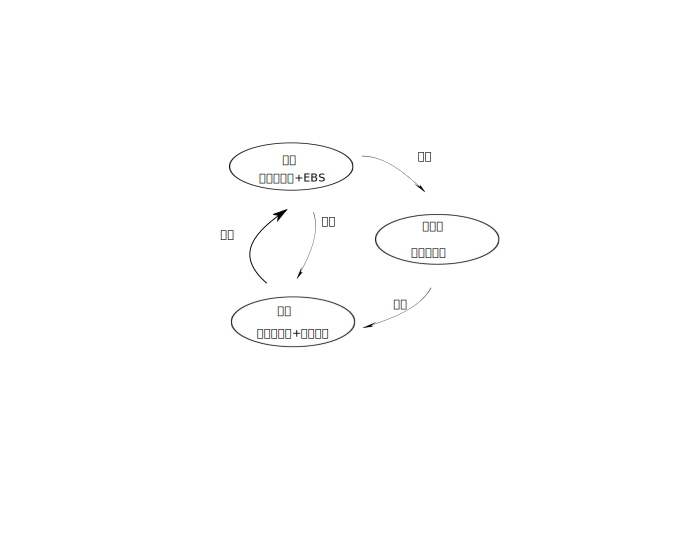
\includegraphics[width=0.6\textwidth]{states}
  \caption{在线服务状态转移图}
  \label{figure:states}
\end{figure}

当新申请的竞价型实例可用时,迁移控制器应该平滑地将在线服务恢复到正常的暖备状态配置。作为一个服务的备援节点,新加入的竞价型实例只需简单的设置为所属服务中对应主节点的备援角色,迁移控制器还需将服务的主节点切换回暖备状态。作为一个服务的主节点,其所属的在线服务应通过进程活迁移转移到该节点,然后服务的暖备互备配置将得以恢复。这个新的主节点需要重新挂载用于持久化数据的EBS,将自身非持久化的的 SSD 本地实例存储作为缓存设备。SSD 本地实例存储同持久化的 EBS 形成时间可控的异步磁盘数据复制配置。在线服务的 IP 地址也要通过 Amazon EC2 API 分配给这个新的虚拟机实例。

当新购买的按需型实例启动完成时,作为一个服务的备援节点所需操作和竞价型实例是相同的。作为一个服务的主节点,用于持久化数据的 EBS 被挂载后不再配置为数据复制方式。SSD 本地实例存储中的脏数据比例不再受限制,写回(Writeback)持久化的 EBS 设备的数据同步操作被挂起。然后在线服务在该节点上恢复并进入没有备援节点的状态。在线服务可能过一段时间后需要从按需型实例迁移回竞价型实例。这种情况下,挂起的磁盘数据复制要先恢复。在 \emph{Gemini} 代理完成 SSD 本地实例存储同持久化 EBS 的同步工作后,再开始进行进程活迁移。由于没有时间上的限制,所有这些在线服务潜在的迁移过程相比强制性迁移都容易完成。

\subsection{虚拟机实例调度器}
当一个竞价型实例被云平台回收时,虚拟机实例调度器将申请新的虚拟机实例替换掉失效的节点。虚拟机实例调度器的任务是在众多可用区中申请一个竞价型实例或购买一个按需型实例。获取新的虚拟机实例在策略上应同时考虑成本效率和服务可用性两个因素。除了在被动的情况下获取新的虚拟机实例,虚拟机实例调度器也会出于成本优化的考虑主动在竞价型实例和按需型实例间切换。在调度策略上主要包括竞价设定和可用区选择两部分。

Cloud Schduler \cite{He:2015:CCH:2749246.2749275} 给出了两个设定竞价的策略:一个是保守型(Reactive)策略,将竞价设为和按需型实例相同的价格;一个是主动型(Proactive)策略,将竞价设为按需型实例价格的 $k$ 倍,$k > 1$。保守型策略当竞价型实例高于按需型实例价格时需要进行服务的强制性迁移。主动型策略当竞价型实例高于按需型实例价格但没有超过设定的竞价情况下不会触发强制性竞价型实例回收,可以主动地申请新的虚拟机实例并将在线服务迁移到新的节点上。主动型策略能一定程度上减少因竞价型实例被回收而发生的强制性服务迁移次数,从而提升冷备配置下的服务可用性。由于 \emph{Gemini} 使用暖备机制已经解决了强制性的不可用问题,使用这两种策略的区别就不是很大了。\emph{Gemini} 选择使用保守型策略控制成本。

在可用区的选择策略上,Cloud Scheduler 采用了最为简单的贪心策略,即根据各个可用区竞价型实例的市场价格选择最低者。\emph{Gemini}则综合考虑了服务可用性和成本两个因素,根据价格趋势和价格稳定性选择可用区。价格的波动可以用近期价格数据的标准差 $\sigma$ 表示。价格趋势可以使用近期价格数据的简单移动平均值(Simple Moving Average)衡量,其计算方式为:
\begin{equation}
SMA = \frac{p_1 + p_2 + \cdots + p_n}{n}
\end{equation}

其中 $p_i$ 表示最近第 $i$ 个周期的竞价型实例市场价格,$SMA$ 即为最近 $n$ 个的竞价型实例市场价格的简单移动平均值。

可用区选择策略如算法 \ref{figure:avz-selection-algo} 所示,步骤大致如下:1)首先列出竞价型云平台的所有可用区,排除掉互备对中另一个节点所在可用区以保证主节点和备援节点的失效独立性。2)然后计算各个可用区最近一段时间竞价型实例市场价格的简单移动平均值 $SMA$ 和标准差 $\sigma$,移除标准差过大的可用区以保证价格平稳减少竞价型实例被回收的情况。3)最后选出平均值最低的可用区,如果该可用区价格低于按需型实例价格则申请竞价型实例,否则在互备对中另一个节点所在可用区购买按需型实例。
\begin{algorithm}
\caption{可用区选择}
\label{figure:avz-selection-algo}
\KwIn{$excluded$, $n$, $T$}
\KwOut{$selected$}
$zones\gets get\_availability\_zones()$\tcp*[r]{获取所有可用区}
\ForEach{$zone \in zones$}
{
  \If{$zone = excluded$}
  {
    $zones.remove(zone)$\;
  }
}
\ForEach{$zone \in zones$}
{
  $avg[zone]\gets SMA(zone.spot\_prices[1..n])$\tcp*[r]{计算简单移动平均}
  $sd[zone]\gets \sigma(zone.spot\_prices[1..n])$\tcp*[r]{计算标准差}
}
\ForEach{$zone \in zones$}
{
  \If{$sd[zone] > T$}
  {
    $avg.remove(zone)$\;
  }
}
$selected\gets min\_key(avg)$\;
\If{$selected.spot\_prices[1] \not< selected.on\_demand\_price$}
{
  $selected\gets excluded$\;
}
\Return{$selected$}
\end{algorithm}

在这个可用区选择算法中,竞价型实例的市场价格标准差 $\sigma$ 和简单移动平均 $SMA$ 值均使用最近 $n$ 个小时的价格历史数据计算得来。$n$ 的值可以根据价格变化频率确定,默认值可设为一天时间(24小时)。可用区选择算法主要考虑备选可用区的价格稳定性和趋势。通过设定一个标准差的阀值 $T$ 可以过滤不稳定的可用区。如果算法返回的可用区同互备对中另一个节点可用区相同则表示应在该可用区购买按需型实例,否则以按需型实例价格作为竞价申请指定可用区的竞价型实例。本章主要工作和重点在于使用轻量级暖备机制提升服务可用性和性能,在可用区选择和竞价设定算法上倾向于简单有效。因此,这里不再引入竞价型实例市场价格的预测模型。在实际使用中,\emph{Gemini} 可以方便地替换虚拟机实例调度器的策略,改用其他竞价算法。

此外,当前地理区域长时间没有可用的竞价型实例时,实例调度器可以选择发起一次地理区域切换。切换地理区域对于那些直接同用户交互的服务可能带来很大的响应请求延迟,对于这类服务最好保持在一个地理区域。另外需要注意的是,EIP 是归属于一个地理区域的。在一个地理区域申请的 EIP 无法分配给另一个地理区域的虚拟机实例。因此,直接同用户交互的服务如果切换地理区域。要求该服务有提供域名给用户访问,同时需要在切换地理区域后,更改DNS记录将域名映射到新的IP地址。同时在原IP所在节点上提供请求转发代理,直至DNS记录更新完成。

另外需要注意的是,由于一个地理区域的 EBS 卷无法在另一个地理区域使用,跨地理区域的互备是不可行的。因此,地理区域切换需要将运行在当前地理区域的服务整体迁移到其他地理区域来使用成本更低的竞价型实例。对于这种跨地理区域的虚拟机实例调度,地理区域选择的方法是基于选择可用区的策略的。如算法 \ref{figure:region-selection-algo} 所示,首先对备选的地理区域使用可用区选择算法。不同之处是每个地理区域要选出两个可用区分别用于部署主节点和备援节点,最后选择两个可用区简单移动平均价格之和最小的地理区域作为目标地理区域。在跨地理区域迁移时,在线服务的 EBS 数据应首先拷贝到目标地理区域。然后,将在线服务的进程迁移到在该地理区域的虚拟机实例上。最后,迁移控制器要对暖备和互备配置进行更新。

\begin{algorithm}
\caption{地理区域选择}
\label{figure:region-selection-algo}
\KwIn{$excluded$}
\KwOut{$selected$}

$regions\gets get\_regions()$\tcp*[r]{获取所有地理区域}
\ForEach{$region \in regions$}
{
  \If{$region = excluded $}
  {
    $regions.remove(region)$\;
  }
}
\ForEach{$region \in regions$}
{
  \tcp*[h]{使用可用区选择算法选出两个可用区}
  $zoneA\gets region.selectAvZ(region.AvZ[1]$
  $zoneB\gets region.selectAvZ(zoneA)$
  $prices[region]\gets zoneA.spot\_prices[1] + zoneB.spot\_prices[1]$\;
}
$selected = min\_key(prices)$\;
\Return{$selected$}
\end{algorithm}

\section{系统评测}
\emph{Gemini} 的原型实现基于 CRIU,Bcache,和 Amazon EC2 APIs。为全面有效的评价这套轻量级暖备方法的有效性,本节在 \emph{Gemini} 原型上进行了一系列的实验。

首先,两个指标被分别用来确认和测量 \emph{Gemini} 的两个组件的可行性和有效性。进程活迁移所需的时间对于 \emph{Gemini} 来说是一个关键指标。它决定了使用活迁移技术在较短的告警时间内完成在线服务迁移的可行性。另一个指标是在 \emph{Gemini} 的时间可控的异步磁盘数据复制配置下 SSD 本地实例存储的 I/O 性能。它是I/O密集型在线服务潜在的性能瓶颈。

两个基准测试集,TPC-W \cite{TPCW:2014} 和 YCSB \cite{YCSB:2014} 负载下的 MongoDB \cite{Mongodb:2014},都被用于在线服务的性能评测。TPC-W 是一个以网上书店为背景的事务型的交易基准测试集,它有一个 Web 服务器层处理顾客请求和一个数据库层维护购买、下订单等交易记录。MongoDB 是一个非常流行的 NoSQL 数据库,它已经被广泛用于各种不同类型的在线服务。YCSB 是一个用于比较各种不同的NoSQL数据库的相对性能的开源测试集规范和 Java 测试程序套件。

最后基于 Amazon EC2 公布的竞价型实例市场价格历史数据,\emph{Gemini} 还进行了一些长期的竞价型云平台上在线服务运行的仿真实验。这些实验评测了 \emph{Gemini} 的可用性和成本效率。

\subsection{微基准测试}

\subsubsection{活迁移时间}
\label{gemini-migrationtime}
这里使用 Amazon EC2 平台 ``us-west-2'' 地理区域不同可用区的两个 ``linux.m3.large'' 竞价型实例作为实验节点。这些实例的网络性能根据 Amazon EC2 的介绍是适中的。使用iperf \cite{Iperf:2014} 测量的结果显示两个竞价型实例的网络带宽约为 600 Mbps。本小节在这样一个典型的云平台配置下测量活迁移服务进程所需时间。

测试中使用一个 \emph{mem-touch} 程序作为准备进行活迁移的服务进程。\emph{mem-touch}程序首先申请一定量的内存然后随机地写这些内存页。本实验测试了不同的内存大小下进程活迁移所需时间。如图 \ref{figure:migrationtime} 所示,内存大小为 2 GB 情况下进程的活迁移时间大约是 25 秒。由于内存页传输是整个活迁移过程中最耗时的部分,进程的活迁移时间主要由它占用的内存大小决定。
\begin{figure}
  \centering
  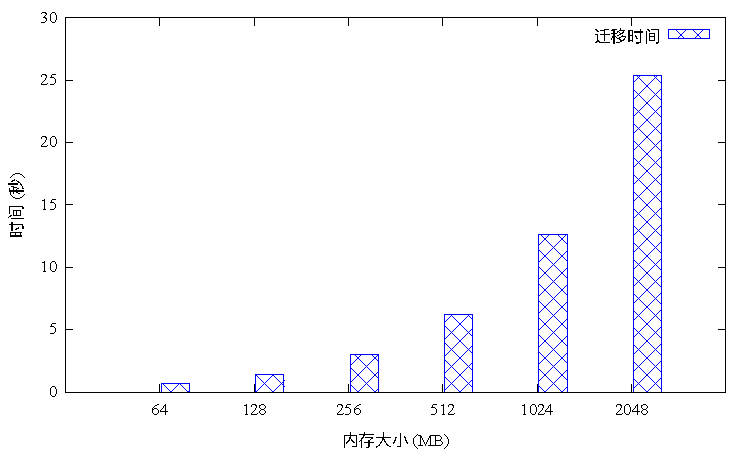
\includegraphics[width=0.9\textwidth]{migrationtime.pdf}
  \caption{活迁移时间开销}
  \label{figure:migrationtime}
\end{figure}

因为 ``linux.m3.large'' 竞价型实例的全部内存有 7.5 GB,在这个配置类型的竞价型实例上的所有在线服务在两分钟的回收告警时间内显然可以完成进程活迁移。对于其他配置类型中内存更大的竞价型实例,其网络带宽也有相应地提升。对于一些超大型(Extra Large)虚拟机实例网络带宽甚至达到了 10 Gbps。因此,可以确定的是 \emph{Gemini} 采用进程活迁移的方式实现在竞价型实例被回收时的服务迁移是可行的。此外,使用进程活迁移的手段还避免了进行定期内存检查点操作带来的性能开销。

\subsubsection{I/O性能}
\emph{Gemini} 同一些其他配置下的 I/O 性能对比是本节的测试目标。这个测试使用了``linux.m3.large''竞价型实例。``linux.m3.large'' 型虚拟机实例的本地实例存储是一个 32 GB 的 SSD。\emph{Gemini} 使用一个同为 32 GB 大小的通用型(General Purpose)SSD EBS 作为后端存储设备。通用型 SSD EBS 可以持续提供 3 IOPS/GB 的基准性能,并支持突发性的 I/O 请求能提供高达 3000 IOPS的性能。实验中使用 fio \cite{FIO:2014},一个灵活的 I/O 测试集工具,来对比 \emph{Gemini} 的时间可控异步磁盘数据复制配置,通常的同步磁盘数据复制配置,以及其他两个存储配置————裸 SSD 本地实例存储和裸通用型 SSD EBS。测试用的文件大小为 2 GB,测试使用 8 个进程提交 16 KB 大小的顺序和随机 I/O 请求。I/O 请求队列深度为 64,测试时间为 60 秒。由于 SSD 本地实例存储和 EBS 卷都是虚拟的存储设备,每个磁盘块第一次访问时可能有 5\% 到 50\% 的性能损失,实验前将待测的存储设备进行了预热处理。
\begin{figure}[]
  \centering
  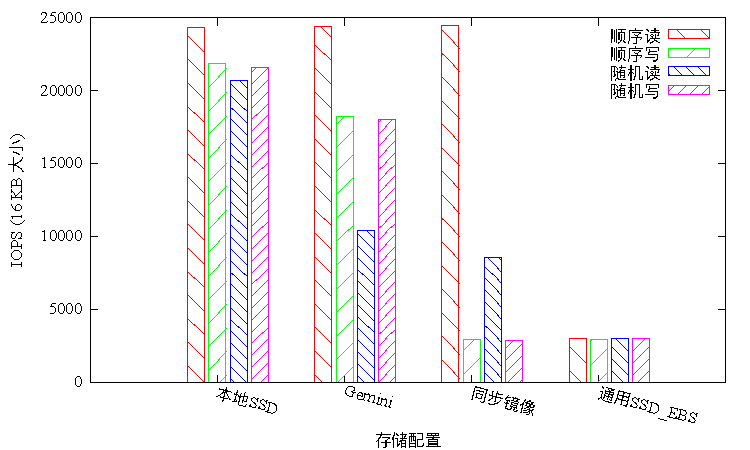
\includegraphics[width=0.9\textwidth]{iops.pdf}
  \caption{不同存储配置下的 IOPS}
  \label{figure:iops}
\end{figure}

图 \ref{figure:iops} 显示了不同存储配置下的 IOPS。毫无疑问,非持久化的 SSD 本地实例存储拥有最好的 I/O 性能。SSD 本地实例存储在顺序或随机读写测试中都可以提供高达 20000 IOPS 的性能。通用型 SSD EBS 的突发 I/O 性能在四个测试中的可达到约 3000 IOPS。这仍要比 SSD 本地实例存储慢 7 倍左右。对于 SSD 本地实例存储和通用型 SSD EBS 设置为同步复制的配置,写性能被限制在通用型 SSD EBS 的 IOPS 吞吐水平。顺序写之后的顺序读性能同 SSD 本地实例存储类似,约 25000 IOPS。随机读测试性能适中,因为只有部分请求由 SSD 本地实例存储处理,未缓存的部分由通用型 SSD EBS 处理。\emph{Gemini} 的时间可控异步磁盘数据复制机制相比同步复制有更好的性能。其顺序和随机写性能接近 SSD 本地实例存储,顺序读性能也接近 25000 IOPS。

\subsection{服务性能基准测试}
测试使用了两个基准测试集,TPC-W 和 YCSB 用于测试不同类型的在线服务在 \emph{Gemini} 框架下的性能。TPC-W 是一个模拟网上书店的交易事务测试集。YCSB 可以生成各种 NoSQL 数据库的工作负载。这里使用 YCSB 评测 SSD 本地实例存储可以多大程度上提升广泛应用于各类在线服务的 MongoDB 的性能。

\subsubsection{TPC-W 基准测试}
TPC-W 基准测试集是一个计算密集的负载。这个测试主要比较 \emph{Gemini} 的轻量级服务迁移方法和基于嵌套虚拟化和虚拟机迁移技术的方法在性能开销上的表现。这里选取了一个 Java Servlets 版本的 TPC-W 实现 \cite{JAVATPCW:2014} 用于测试。其中,Web 应用前端部署在 Apache Tomcat 7 上,数据库后端使用的是 MySQL 5.0。Web 服务器和数据库服务器运行在 ``linux.m3.large'' 竞价型实例上,主要配置为 2 个 VCPU 和 7.5 GB 内存。测试中使用另外的虚拟机实例模拟浏览器请求生成用户访问负载。测试中使用混合型订单(Ordering Mix)负载,其中有 50\% 交互请求为浏览访问,50\% 交互请求为下订单操作。

方便比较,测试在 ``linux.m3.large'' 竞价型实例上运行的 Xen-Blanket \cite{Williams:2012:XVO:2168836.2168849} 嵌套虚拟机管理器中创建了一个嵌套虚拟机。它的配置为 2 个 VCPU 和 7 GB 内存,因为虚拟机管理器也需要使用一部分内存。这并不会带来性能差异,因为 Tomcat 和 MySQL 在 TPC-W 测试中使用的内存量之和远远小于 7 GB。

图 \ref{figure:tpcw} 显示了在不同用户请求压力下 Web 交互的平均响应时间。\emph{Gemini} 的表现从 50 个到 400 个并发访客测试一直好于基于嵌套虚拟化的解决方法。\emph{Gemini} 的性能开销非常低,因为在线服务正常运行时 \emph{Gemini} 不进行内存检查点任务。而基于嵌套虚拟化的 Cloud Scheduler 在运行 TPC-W 基准测试集负载时则存在 30\% 到 45\% 的性能开销。
\begin{figure}[]
  \centering
  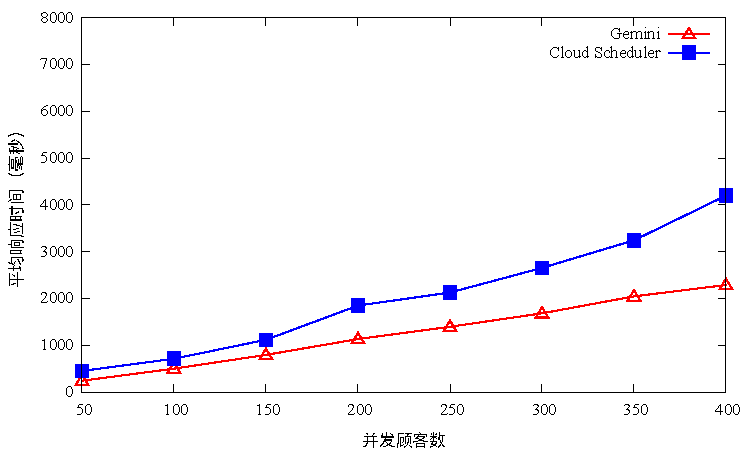
\includegraphics[width=0.9\textwidth]{tpcw.pdf}
  \caption{TPC-W 测试集中不同请求压力下的平均响应时间}
  \label{figure:tpcw}
\end{figure}

对于计算密集的工作负载,如此大的性能开销意味着为提升性能到原来的水平必须再使用一个虚拟机实例。使用轻量级的进程迁移技术显然是一个更好的选择。此外,\emph{Gemini} 基于暖备的故障转移方式消除了新的虚拟机实例启动所需的时间。\emph{Gemini}可以将全部两分钟回收告警时间用于服务迁移,包括同步磁盘数据更新和进程迁移。当活迁移可以安全地在告警时间内完成,内存检查点操作就没有必要了,这进一步减少了性能开销。

\subsubsection{YCSB 负载下 MongoDB 性能测试}
本节选择了两个典型的 YCSB 负载来测试 MongoDB 的性能。一个是更新较多的负载,有 50\% 的读操作和 50\% 的更新操作。另一个是读为主的负载,有 95\% 的读操作和 5\% 的更新操作。所有请求在数据库的键名(Key)空间呈均匀分布。实验仍然在 ``linux.m3.large'' 竞价型实例上进行,这个类型的节点有 32 GB 的 SSD 本地实例存储。一个同样 32 GB 大小的通用型 SSD EBS 用于备份存储。\emph{Gemini} 以时间可控的方式复制 SSD 本地实例存储的磁盘数据更新到 SSD EBS。更新频繁和以读为主两类 YCSB 负载在 \emph{Gemini} 配置下和通用型 SSD EBS 下的吞吐和延迟性能数据如图 \ref{figure:ycsba} 和图 \ref{figure:ycsbb} 所示。
\begin{figure}[]
  \centering
  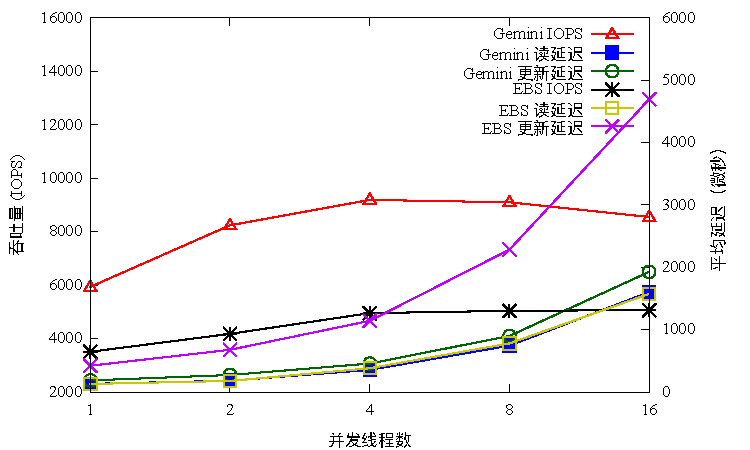
\includegraphics[width=0.9\textwidth]{ycsba.pdf}
  \caption{MongoDB 在更新频繁负载下的吞吐性能}
  \label{figure:ycsba}
\end{figure}

\emph{Gemini} 在更新频繁的负载下可以达到通用型SSD EBS约两倍的 IOPS 吞吐。在两类负载下,\emph{Gemini} 的读延迟和通用型 SSD EBS 几乎相同。\emph{Gemini} 大幅减少了写延迟,在更新频繁的负载压力下写延迟相比通用型 SSD EBS 的性能改善有约 2.5 倍之多。如图 \ref{figure:ycsbb}所示,对于以读为主的负载,\emph{Gemini} 只有相对 SSD EBS 至多 18\% 的 IOPS 吞吐性能提升。这是因为 MongoDB 对大部分读请求的处理有效利用了内存中的缓存数据。
\begin{figure}[]
  \centering
  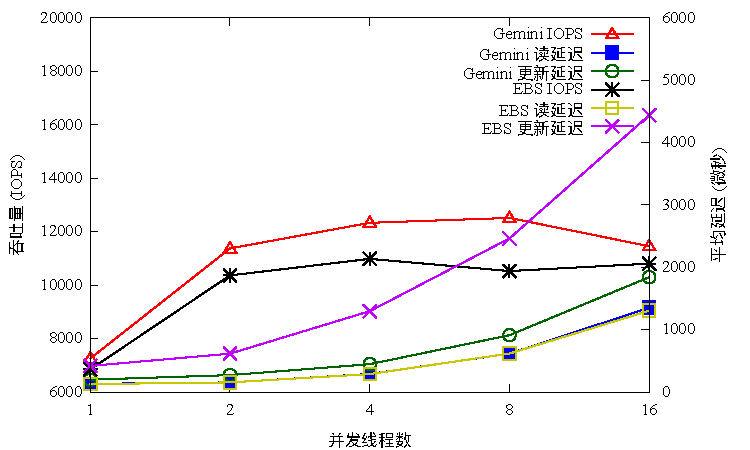
\includegraphics[width=0.9\textwidth]{ycsbb.pdf}
  \caption{MongoDB 在以读为主负载下的吞吐性能}
  \label{figure:ycsbb}
\end{figure}

\subsection{成本与可用性分析}
根据虚拟机实例的启动时间,服务迁移时间,以及 Amazon EC2 的竞价型实例市场价格历史数据,本节进行了长期(约 1 个月时间)的在线服务运行仿真。仿真参数包括实测的虚拟机实例启动时间和服务迁移时间等,保证了仿真结果的有效性。按需型实例和竞价型实例的启动时间数据由 Mao 等人 \cite{Mao:2012:PSV:2353730.2353859} 收集。不同内存大小的进程迁移时间已在 \ref{gemini-migrationtime} 小节中作为一个指标测量过。

仿真实验中的在线服务为 TPC-W 基准测试集中的网上书店。网上书店的架构包括一个 Web 服务器和一个数据库服务器,各使用一个竞价型实例。在 \emph{Gemini} 框架中,这两个节点被迁移控制器组织成一个互备对。这是 \emph{Gemini} 框架下最基本的应用案例。实验中分别使用小型、中型、大型、超大型竞价型实例的历史价格数据进行这样一个在线服务的仿真。通过这些仿真实验,使用 \emph{Gemini} 在竞价型云平台上提供在线服务的成本和可用性得以评测。

因为虚拟机实例调度器根据近期竞价型实例市场价格数据的标准差(Standard Deviation)和简单移动平均值(Simple Moving Average)选择可用区,这个可用区选择策略被表示为 ``SD-SMA''。另一个简单的贪心策略是选择当前竞价型实例市场价格最便宜的可用区,可以表示为``Greedy''。在 \emph{Gemini} 中,竞价价格被设置为相应按需型实例的价格。根据 He 等人的介绍 \cite{He:2015:CCH:2749246.2749275},作为对照的 Cloud Scheduler 策略中竞价被设定为按需型实例价格的 4 倍以期减少竞价型实例回收的发生。

仿真测试中各种策略的服务不可用性如图 \ref{figure:cost} 所示,\emph{Gemini} 框架的服务可用性在小型、中型、大型、超大型虚拟机实例下都比 Cloud Scheduler 好至多达一个数量级。因为在 \emph{Gemini} 的高可用配置中,活迁移可以在收到回收告警通知后立即开始。而且,在线服务只有在活迁移过程中的冻结时间处于不可用状态。通过使用 Pre-copy 迁移方式,冻结时间可以降低到数十毫秒。然而,基于冷备的框架在强制性迁移时必须首先获取一个新的虚拟机实例。虚拟机实例的启动时间严重影响了在线服务在这一场景下的可用性。设置一个比按需型实例价格更高的竞价在超大型虚拟机实例的案例下取得了较好的效果,因为这一类型的虚拟机实例经常波动到超过按需型实例价格的程度。
\begin{figure}[]
  \centering
  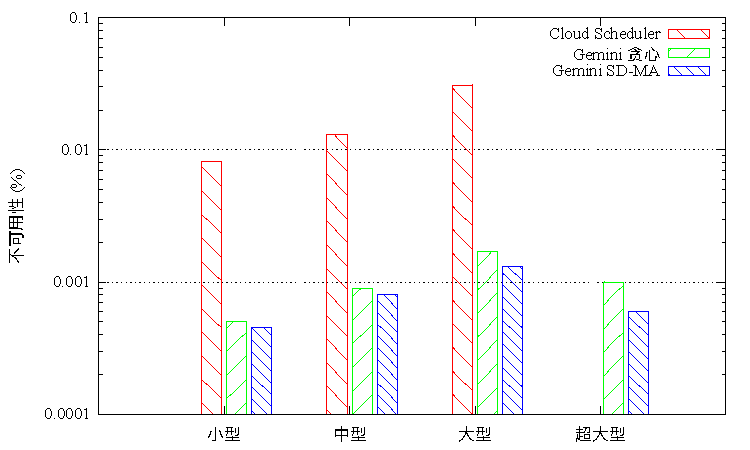
\includegraphics[width=0.9\textwidth]{availability.pdf}
  \caption{单地理区域不可用性比较}
  \label{figure:unavailability}
\end{figure}

``SD-SMA'' 策略相比 ``Greedy'' 策略减少了强制性迁移的次数。这一策略在大多数情况下通过选择价格稳定的可用区取得了更好的可用性。相对地,如图 \ref{figure:cost} 所示,这个策略在一些情况下成本更高。这是因为最便宜的可用区可能是不稳定的。图 \ref{figure:cost} 显示了在 ``us-west2'' 地理区域使用不同框架提供在线服务的归一化成本。基线是使用按需型实例提供同一在线服务的成本。\emph{Gemini} 的成本大致只有基线的 14\% 到 23\%。这同 Cloud Scheduler 接近。
\begin{figure}[]
  \centering
  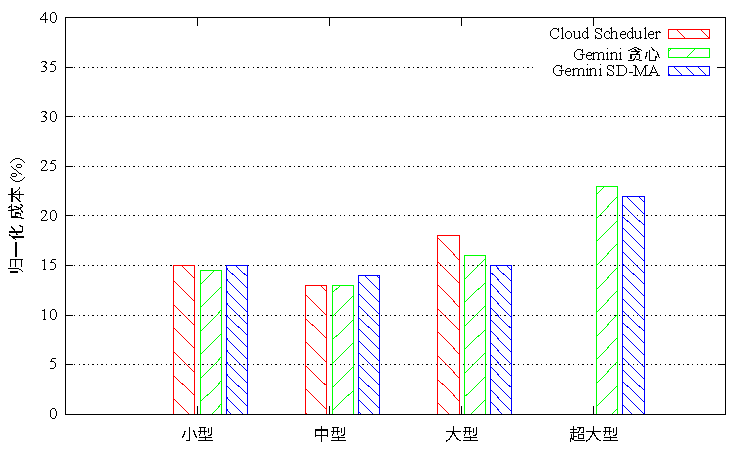
\includegraphics[width=0.9\textwidth]{cost.pdf}
  \caption{单地理区域的成本比较}
  \label{figure:cost}
\end{figure}

实验还进行了多地理区域场景下的仿真。只有处理美国的三个地理区域:``us-west1'',``us-west2'',``us-east'' 在实验中被使用。图 \ref{figure:unavailabilitymulti} 和 \ref{figure:costmulti} 显示了在多个地理区域中利用 \emph{Gemini} 等框架提供在线服务的成本和可用性情况。\emph{Gemini} 的可用性相比单地理区域情况有所提升。因为多地理区域有更多的可用区作为候选可以使在线服务运行在竞价型实例市场价格更稳定的可用区上。然而,多地理区域下 ``Greedy'' 策略在某些情况下的不可用性有所增加。这是由于便宜的可用区可能价格不稳定,在多个地理区域中贪心地选择最便宜的可用区在线服务可能经历更多的强制迁移。
\begin{figure}[]
  \centering
  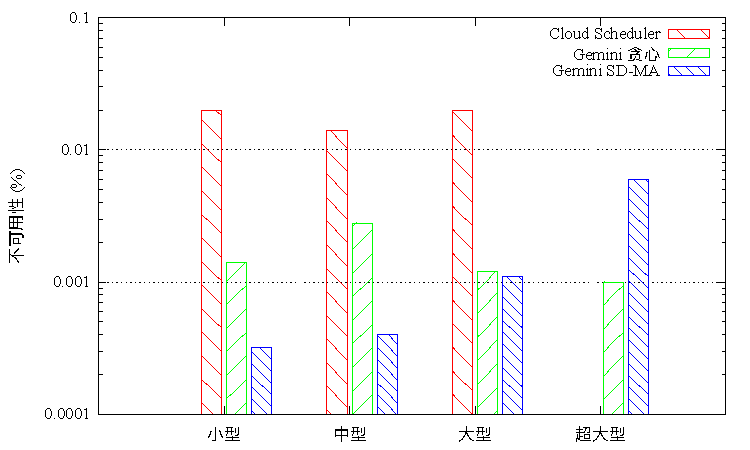
\includegraphics[width=0.9\textwidth]{availabilitymulti.pdf}
  \caption{多地理区域不可用性比较}
  \label{figure:unavailabilitymulti}
\end{figure}

\begin{figure}[]
  \centering
  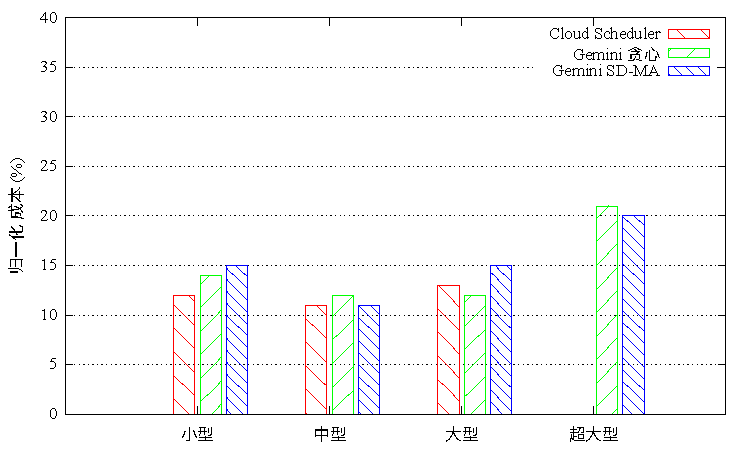
\includegraphics[width=0.9\textwidth]{costmulti.pdf}
  \caption{多地理区域的成本比较}
  \label{figure:costmulti}
\end{figure}

如图所示,在多地理区域场景下提供在线服务的成本效率在大多数情况下得以改善。\emph{Gemini} 的成本在几种不同的实例类型下低至基线的 11\% 到 22\%。使用 ``SD-SMA'' 策略的成本略高于 ``Greedy'' 策略,但获得了显著的可用性提升。

\section{本章小节}
\emph{Gemini}提供了一个轻量级的使用竞价型实例运行在线服务的高可用方法。同现有方法相比,\emph{Gemini} 通过基于暖备的故障转移方式消除了强制性不可用的情况。而且 \emph{Gemini} 使用轻量级的进程活迁移机制减少了服务运行和迁移过程中的性能开销。出于性能方面的考虑,在 \emph{Gemini} 的设计中允许在线服务使用高性能的 SSD 本地实例存储。\emph{Gemini} 负责从 SSD 本地实例存储复制磁盘数据更新到 EBS 以实现数据持久化。为保证可以在回收告警时间内完成数据同步同时提供最好的 I/O 性能,\emph{Gemini} 使用了时间可控的异步磁盘数据复制机制。通过组合使用几个系统级技术,\emph{Gemini} 提供了在不可靠的竞价型实例上运行在线服务的故障转移机制。当互备对中的一个节点被云平台回收时,\emph{Gemini} 通过备用节点保证服务可用性,同时从云平台获取一个虚拟机实例以恢复原来的高可用配置。

在\emph{Gemini}原型系统上的一系列的实验验证和评测了该方法的有效性。在 TPC-W 基准测试集下,\emph{Gemini} 相比基于嵌套虚拟化的方法可以减少 30\% 到 45\% 的性能开销。在 YCSB 更新频繁的负载下,\emph{Gemini} 框架下的 MongoDB 可以获得大约两倍的吞吐性能提升和 2.5 倍的写延迟性能提升。基于 Amazon EC2 平台 已公布的竞价型实例历史价格数据的长期在线服务仿真显示:\emph{Gemini} 相比之前的方法在可用性上实现了近一个量级的提升,以及相比使用按需型实例五到六倍的成本节省(和现有方法相近)。